%%% Local Variables:
%%% mode: latex
%%% TeX-master: t
%%% End:

\chapter{基于Uppaal的中断模型}
\label{cha:intr}

\section{Uppaal中的模型组成}
\label{sec:model_combine}	
一套Uppaal模型由以下三部分组成。
\begin{itemize}
	\item \emph{声明}:整个模型系统中共有的声明,可以是变量或函数。在整个
	系统中都可以访问。
	\item \emph{自动机模板}:各类自动机的通用模板,一个模型系统可以有多个
	模板,一个模板在系统中可以对应多个实例。
		\begin{enumerate}[(1)]
			\item \emph{声明}:模板内部的变量或函数,只有本模板的实例可
			以访问。
			\item \emph{位置}:时间自动机的位置,每个位置可以有初始(
			initial),紧急(urgent),关键(committed)。关键位置与紧
			急位置上,模型中的时钟都停止。不同的是,当有自动机在关键位置时,
			在下一个状态迁移必须从某一个关键位置发出。
			\item \emph{变迁}:位置到位置的迁移。变迁包含选择(select)
			、条件(guard)、同步(sync)、更新(update)四个属性。其中,
			同步和更新是同时发生的。
		\end{enumerate}	
	\item \emph{模型声明}:定义组成系统的模板实例。
\end{itemize}

\section{基本中断模型}
\label{sec:basic}
通常,在我们接触到的非实时性电脑环境中,中断的行为就是符合一个中断的基本模型。其
行为模式就是简单的抢占当前线程,在执行结束之后恢复上下文继续执行被抢占的线程。

\begin{figure}[H]
	\centering
	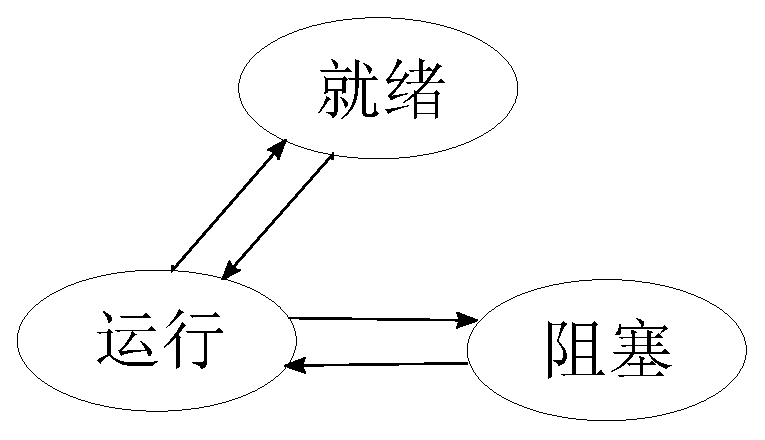
\includegraphics[width=0.5\textwidth]{thread_states}
	\caption{单个线程的状态}
	\label{fig:thread_state}
\end{figure}

中断处理程序的行为,与多线程程序研究中的线程行为十分相似。我们对中断模型的构建就
参考了多线程程序中的线程模型。如图~\ref{fig:thread_state} 所示,通常,一个线程
会被刻画为以下三个状态。
\begin{itemize}
	\item \emph{就绪}:线程可以运行但是当前并不占有CPU。
	\item \emph{运行}:线程正在运行。
	\item \emph{阻塞}:线程在等待处理器以外的资源,暂时无法运行。
\end{itemize}
由于绝大部分多线程程序研究的场景中,并不关心线程产生和终止。换言之,线程在这类应
用场景里直接存在,且永不终止。中断研究中,一个通常具有一个从产生到终止的完整周期
。而且,一个中断并非只触发一次,因此一个可能重复多次上述周期。这与传统的多线程程
序研究是不同的。所以针对一个,我们类比线程再加以修改可以得到如图~\ref{fig:interrupt_state} 
所示的状态机。每个状态的含义如下。

\begin{figure}[H]
	\centering
	
\includegraphics[width=0.5\textwidth]{interrupt_states}
	\caption{单个的状态}
	\label{fig:interrupt_state}
\end{figure}

\begin{itemize}
	\item \emph{无中断}:当前中断没有触发。
	\item \emph{就绪}:中断触发但是有优先级更高的中断在执行。
	\item \emph{运行}:正在运行。
	\item \emph{阻塞}:被优先级更高的中断打断。
\end{itemize}

在多线程的场景中,线程之间的切换往往由线程调度器掌管。线程调度器不是硬件,而是一
段代码,负责实现线程的调度算法。时间片轮转,优先级不同的线程之间的抢占,甚至是线
程优先级的动态变化,都由线程调度器实现。一般而言,线程调度器是系统内核的一重要组
成部分。线程调度器工作的基础就是如图~\ref{fig:thread_table} 所示的线程表结构。
线程表通常是一个二维的表,由系统所支持的线程优先级数构成表的行,每一行内是属于该
优先级的所有线程。通常情况下,系统中会有一个就绪线程表和一个阻塞线程表,当前线程
不在任何一个表中。所有的线程调度算法其实都是对这个表的调整。

\begin{figure}
	\centering
	
\includegraphics[width=0.6\textwidth]{thread_table}
	\caption{线程表}
	\label{fig:thread_table}
\end{figure}

相比而言,多中断场景比多线程场景简单许多。通常情况下,一个中断优先级对应一个中断
处理程序。所以,中断处理程序的组织形式也是一个表,但是从二维降到了一维。在大部分
文档中,这个表被称为中断向量表(Interrupt Vector Table),如图~\ref{fig:interrupt_vector_table} 
所示。中断向量表中的每个表项被称为一个中断向量(Interrupt Vector),指代一个中
断处理程序。在实现时,一个中断向量通常是一个函数指针,指向某个函数,该函数的内容
就是中断处理。因此,不同于多线程场景中,一个线程优先级可以对应多个线程,如图~
\ref{fig:thread_table}中所示,一个中断优先级对应最多一个中断。中断优先级是由CPU
或外部中断控制器等硬件决定的,实际使用时可能用不到所有的优先级,因此会有大量的中
断向量表项为空。

\begin{figure}[H]
	\centering
	
\includegraphics[width=0.25\textwidth]{interrupt_vector_table}
	\caption{中断向量表}
	\label{fig:interrupt_vector_table}
\end{figure}

除了维数降低,中断向量表相比于线程表而言,还有两个不同点。其一,一般而言,中断向
量表在系统初始化完成以后就不再变化。这里的变化指的是已有的中断的优先级变化,即已
有中断在中断向量表中的位置变化。部分操作系统或裸机程序会有在运行时注册或注销中断
的行为,但是从来没有过更改一个现有中断优先级的行为。换言之,在运行时,中断向量表
可以增加或删除表项,但不会更改表项。\footnote{这是一条编程准则。事实上,只要有足
够的权限,更改中断向量表项的操作是被允许的,因而也是可以完成的。只不过大家都不这
么做。}

其二,中断向量表只有一份,包含了所有的中断,不论其当前状态如何。以线程表而言,系
统中可能有两份甚至多份线程表,分别记录不同状态下的线程。除了笼统地将阻塞线程做成
一张线程表,还有一些实现是将请求同一个锁变量的阻塞线程做成一张单独的表。在该实现
下,系统内会同时存在$L+1$张线程表($L$代表系统中锁的数量),另外还有一个当前线程
不在任何线程表内。

到此,一个概念中最基本的中断模型就形成了。中断处理程序状态机如图~\ref{fig:interrupt_state} 
所示,中断间的组织如图~\ref{fig:interrupt_vector_table} 所示。

\subsection{通用的硬件实现}
\label{subsec:basic_hardware}

为了更加忠实地构建模型,我们需要了解中断的实现。因为基本中断模型完全是由硬件实现
的,了解硬件实现的细节能帮我们掌握更多细节,这有助于帮助我们针对遇到的问题进行合
适的抽象。另一方面,虽然中断的实现完全依赖硬件,但是各个硬件平台在实现上述基本中
断机制的方法大同小异,因此本节将介绍一种通用的实现。

中断的硬件实现最主要两个部分是的中断控制器和中断向量表。

中断控制器在\ref{sec:intr}节有简要的介绍。无论是CPU内部还是外部的控制器,其控
制逻辑都是类似的。通常,CPU会有一个或多个指示当前各种状态的STATUS寄存器。STATUS
寄存器中有一位表示是否有中断需要处理,我们称其为中断标志位。CPU在每一个指令周期
之后会检查中断标志位是否置位,如果置位,CPU会和中断控制器通信获取中断号,然后保
存当前上下文,程序计数器(PC)加载中断向量表中对应表项所指向的中断处理程序地址,
开始执行中断程序。进入中断处理时,CPU还会修改STATUS寄存器中的其他的位以表示它现
在正在处理中断。相应的,中断控制器上会有寄存器修改指示当前所有的中断的状态。在接
受新的中断触发信号之后,中断控制器内部的判定逻辑会决定该中断是否可以立即抢占CPU,
进而决定是否需要将CPU的STATUS寄存器中的中断标志位置位。

中断向量表简单许多。通常,中断向量表是在内存中一块独立的区域。在许多平台上,这块
区域从0x0000\footnote{这里用16位数只是举例,表示在内存首地址。如果在32位或64位
平台,地址应该写成0x0000 0000和0x0000 0000 0000 0000}开始。因为CPU会根据一个
中断向量号来查找对应表项,因此中断向量表的基地址完全由CPU的硬件实现规定。部分CPU
允许在系统初始化的时候重新选择中断向量表的基地址,其原理就在于在这些CPU寻址中断
处理程序时,中断向量表基地址是从一个内部寄存器中取出。通过特定的汇编语句可以修改
该寄存器的值,这就完成了中断向量表基地址的修改。在硬件上电启动之前,中断向量表里
的表项并未被赋值。上电之后,在初始化时,由软件给中断向量表各个用到的表项填上对应
的值,通常是各中断处理函数的函数指针。

\subsection{Uppaal中的基本中断模型}
\label{subsec:basic_uppaal}

在构建中断模型之前,我们首先需要对中断场景做一些必要的简化和抽象,同时辅以合理的
假设,以保证我们最终的问题可解。本文的出发点是多中断相互作用下的中断实时性研究。
中断处理程序的语义我们并不关心,因此中断处理程序的语义可以被忽略。一个中断处理程
序就是一个如图~\ref{fig:interrupt_state} 所示的状态机。而另一方面,我们需要中断
处理的时间。这个时间完全依赖硬件平台,同样的代码换另一套硬件时间会完全不一样,虽
然直观上不同的中断处理的相对时间在不同硬件平台应该保持一致。但事实并非如此。如定
义~\ref{def:intr_time} 中所示,我们需要的中断处理时间$T$。$\tau_1$和$\tau_3$
在同一个硬件平台上针对不同的中断,理论上是一样的。但是$\tau_1$和$\tau_3$在不同
的硬件平台上不一样,这一点很容易理解。$\tau_2$在不同的硬件平台上也不一定会保持同
样的相对关系,也就是说,两段中断处理程序代码在两个不同的硬件平台A和B上的运行时间
的比值$\tau_{2A}/\tau_{2B}$不一定保持一致。这完全依赖于针对两个硬件平台的编译过
程。

\begin{definition}
	中断处理的时间$T$
	\label{def:intr_time}
	\begin{equation}
		T = \tau_1 + \tau_2 + \tau_3
	\end{equation}
	
	$\tau_1$:CPU从检测到中断信号开始到PC跳转到中断处理程序的时间。
	
	$\tau_2$:中断处理程序代码的运行时间。
	
	$\tau_3$:CPU恢复上下文,PC跳转回原执行流的时间。
\end{definition}

因此,在不同的硬件平台,中断处理的时间并没有严格的规律可循,针对一个新的硬件平,
中断处理的时间只能通过测试获得。我们在构建中断模型时,需要将中断处理时间纳入模型
中。又因为中断处理时间只能通过测试获得,我们需要将其参数化以保证我们的模型适用性
更好。

除了中断处理时间$T$,我们还应该关心另一个时间 \pozhehao 中断响应耗时$T^\prime$。
注意定义~\ref{def:intr_last} 中开始时刻是中断控制器接收到中断信号的时刻而不是
CPU的检测到中断信号。我们在接下来的建模中会解释这个区别。

\begin{definition}
	中断响应耗时$T^\prime$指从中断控制器收到中断信号时刻开始到当前时刻消耗的时间。
	\label{def:intr_last}
\end{definition}

接下来,一个重要的元素是优先级。如上文所说,中断优先级在运行时保持不变。但是每个
优先级只有一个中断。模型中所有的中断实例都会有一个独特的中断优先级。因此,我们也
可以将中断优先级与中断ID视作同一个变量。事实上,我们也是这么做的。另一方面,由于
对每个中断来说,其优先级都是独一无二的,因此我们无法将优先级作为一个模型中共有的
部分。如同上述的中断处理时间$T$,中断优先级在建模时只能作为一个参数加入Uppaal模
板之中。

以上只描述了~\ref{subsec:basic_hardware} 节中的中断向量表中的内容,模型中还需
要加入中断控制器的内容。得益于Uppaal的模块同步机制,中断控制的机制可以利用中断模
型间的通信来完成。虽然这样的建模与硬件实现有着本质上的不同,中断不再受到一个管理
者实体控制,而是根据一些规则实行了“民主协商自治”。但是,由于“自治”的规则与管理控
制的规则完全相同,因此实现的效果是相同的。

至此,我们可以在Uppaal中构建基本中断的模型了。按照~\ref{sec:model_combine} 节
中介绍的顺序,现在分别展示模型的各个部分。

\subsubsection{声明}
\label{subsubsec:basic_decl}

如图~\ref{fig:basic_decl} 所示,第1行定义了中断优先级的总数,代码中的数字只是
一个例子。第2行定义了一个数据类型,它的作用就如它的名字一样,中断ID。同时,它也
是中断的优先级,数字越小,优先级越高。优先级最高的是0号中断。接下来定义信道,第
3行定义了一组通信信道,分别对应每个中断。第4行定义了两个广播信道。普通信道的信号
只能有一个发送者,一个接收者;广播信道则有一个发送者和多个接收者。普通信道的作用
是用于环境触发特定中断,而广播信道就用来实现抢占,或者由被抢占重新占有CPU的效果。
第5行定义了一个布尔变量数组,模拟ISR(Interrupt Service Register)寄存器。这个
寄存器通常是中断控制器的重要组成部分,在不同硬件平台上有不同的名字,甚至可能代表
了多个寄存器。它的作用指示当前有哪几个中断需要处理,包含正在处理的中断。如果某一
个中断尚未处理结束,即该寄存器某一位置位时,同一中断的下一个实例又触发了,在基本
中断模型中,会被忽略。第8-17行定义了一个函数用来获取当前存在的优先级最高的中断的
优先级(或者说ID)。但是,如果ISR数组里的值都是False,即当前没有任意一个中断需要
处理,那么该函数返回N。优先级N不对应任何一个中断,我们可以认为优先级N对应的是普
通代码。

\begin{figure}[H]
	\centering
	\begin{lstlisting}
	const int N = 7;
	typedef int[0, N-1] intr_id; 
	chan intr[intr_id];
	urgent broadcast chan prompt, resume;
	bool ISR[intr_id] = {false, false,false,
					false,false,false,false};
	
	typedef int[0,N] Pri;
	Pri get_highest_pri(){
		meta int i;
		for(i = 0; i < N; i++){
			if(ISR[i]){
			return i;
			} 
		}
		return N;
	}
	\end{lstlisting}
	\caption{基本中断模型:声明}
	\label{fig:basic_decl}
\end{figure}

\subsubsection{基本中断模板}

\begin{figure}
	\centering
	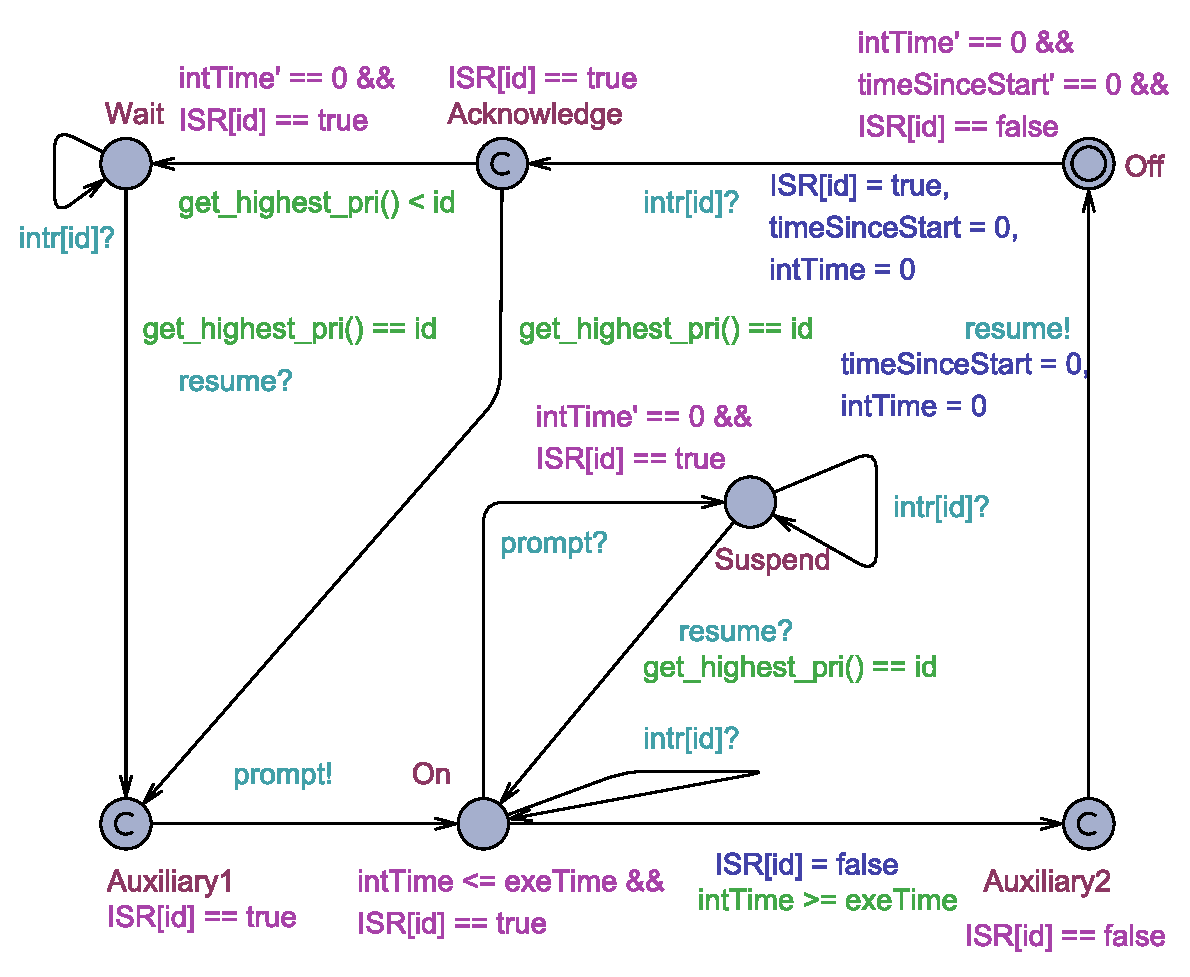
\includegraphics[width=0.9\textwidth]{Interrupt_basic}
	\caption{基本中断:状态机}
	\label{fig:interrupt_basic}
\end{figure}

基本中断的状态机如图~\ref{fig:interrupt_basic} 所示,在这个状态机的状态在Uppaal
中称为位置(Location),以便于整个模型的状态相区分。该模板的内部声明、参数、位置
和变迁的说明分别如表~\ref{tab:basic_intr_decl},表~\ref{tab:basic_intr_para},
表~\ref{tab:basic_intr_loc},表~\ref{tab:basic_intr_mov} 所示。这里,我们定义

\begin{definition}
	中断实际处理时间$t$,指从CPU接收到本中断信号开始到当前时刻的时间。
\end{definition}

注意,表~\ref{tab:basic_intr_mov} 中并没有选择一列,因为在该模板中,所有的位置
变迁都没有规定选择属性。

\begin{table}[htb]
	\centering
	\caption{基本中断模板:内部声明}
	\label{tab:basic_intr_decl}
	\begin{tabularx}{\linewidth}{p{7em}p{5em}X}
		\toprule[1.5pt]
		{\heiti 名称} & {\heiti 类型} & {\heiti 含义}\\
		\midrule[1pt]
		intTime & clock & 中断实际处理时间$t$ \\
		\midrule[0.5pt]
		timeSinceStart & clock & 中断响应耗时$T^\prime$ \\
		\bottomrule[1.5pt]
	\end{tabularx}
\end{table}

\begin{table}[htb]
	\centering
	\caption{基本中断模板:参数}
	\label{tab:basic_intr_para}
	\begin{tabularx}{\linewidth}{p{7em}p{5em}X}
		\toprule[1.5pt]
		{\heiti 名称} & {\heiti 类型} & {\heiti 含义}\\
		\midrule[1pt]
		id & int & 中断号,也是中断优先级 \\
		\midrule[0.5pt]
		exeTime & int & 中断处理时间$T$ \\
		\bottomrule[1.5pt]
	\end{tabularx}
\end{table}

\begin{longtabu} to \linewidth {p{5em}p{5em}p{13em}X}
	\caption{基本中断模板:位置}
	\label{tab:basic_intr_loc}\\
	\toprule[1.5pt]
	{\heiti 名称} & {\heiti 附加属性} & {\heiti 约束} & {\heiti 含义}\\
	\midrule[1pt]
	\endfirsthead
	\multicolumn{4}{c}{续表~\thetable\hskip1em 基本中断模板:位置}\\
	\toprule[1.5pt]
	{\heiti 名称} & {\heiti 附加属性} & {\heiti 约束} & {\heiti 含义}\\
	\midrule[1pt]
	\endhead
	\hline
	\multicolumn{4}{r}{续下页}
	\endfoot
	\endlastfoot
	Off & 初始位置 & intTime和timeSinceStart保持静止,ISR对应位为false & 
	初始位置,当前没有该中断\\
	\midrule[0.5pt]
	Acknowledge & 关键位置 & ISR对应位为true & 中断控制器接收到中断信号\\
	\midrule[0.5pt]
	Wait & & intTime保持静止,ISR对应位为true & 当前有优先级更高的中断在运
	行,本中断等待。\\
	\midrule[0.5pt]
	Auxiliary1 & 关键位置 & ISR对应位为true & 为表达Wait和Acknowledge到On
	的语义设置的辅助位置\\
	\midrule[0.5pt]
	On & & intTime不超过exeTime,ISR对应位为true & 中断正在被处理 \\
	\midrule[0.5pt]
	Suspend & & intTime静止,ISR对应位为true & 中断被更高优先级抢占CPU \\ 
	\midrule[0.5pt]
	Auxiliary2 & 关键位置 & ISR对应位为false & 为表达On到Off的完整语义设置
	的辅助位置\\
	\bottomrule[1.5pt]
\end{longtabu}

\begin{longtabu} to \linewidth {p{5em}p{5em}XXXX}
	\caption{基本中断模板:变迁 }
	\label{tab:basic_intr_mov}\\
	\toprule[1.5pt]
	{\heiti 迁出位置} & {\heiti 迁入位置} & {\heiti 条件} & {\heiti 同步} & 
	{\heiti 更新} & {\heiti 含义}\\
	\midrule[1pt]
	\endfirsthead
	\multicolumn{6}{c}{续表~\thetable\hskip1em 基本中断模板:变迁}\\
	\toprule[1.5pt]
	{\heiti 迁出位置} & {\heiti 迁入位置} & {\heiti 条件} & {\heiti 同步} & 
	{\heiti 更新} & {\heiti 含义}\\
	\midrule[1pt]
	\endhead
	\hline
	\multicolumn{6}{r}{续下页}
	\endfoot
	\endlastfoot
	Off & Acknowledge & & 接收到中断信号 & ISR对应位置位,时钟清零 & 中断控
	制器接收到中断信号\\
	\midrule[0.5pt]
	Acknowledge & Wait & 本中断优先级不是最高 & & & 当前有更高优先级的中断存
	在,本中断等待\\
	\midrule[0.5pt]
	Wait & Auxiliary1 & 本中断优先级最高 & 接收到resume信号 & &  高优先级的
	中断执行完毕,本中断得到CPU\\
	\midrule[0.5pt]
	Acknowledge & Auxiliary1 & 本中断优先级最高 & & & 本中断优先级最高,准备
	执行\\
	\midrule[0.5pt]
	Auxiliary1 & On & & 发送prompt信号 & & 当前中断获得CPU,打断其他正在被处
	理的中断\\
	\midrule[0.5pt]
	On & Suspend & & 接收到prompt信号 & & 当前中断被更高优先级的中断打断\\
	\midrule[0.5pt]
	Suspend & On & 本中断优先级最高 & 接收到resume信号 & & 高优先级的中断执
	行完毕,本中断得到CPU\\
	\midrule[0.5pt]
	On & Auxiliary2 & 中断实际处理时间$t$超过中断处理时间$T$ & & ISR对应位
	复位 & 中断执行结束\\
	\midrule[0.5pt]
	Auxiliary2 & Off & & 发送resume信号 & 时钟清零 & 通知其他中断获取CPU\\
	\bottomrule[1.5pt]
\end{longtabu}

\subsubsection{环境模板}
\label{subsubsec:basic_env}

环境实例的作用是提供一个中断触发源。在本模型中,由于没有其他的规定,中断的触发方
式为随机触发。如图~\ref{fig:evn_basic} 所示,环境模板没有内部声明,只有一个位
置,无实际意义,其存在是为了在变迁中随机向intr[0]至intr[N-1]的信道中发送一个信
号。

\begin{figure}[H]
	\centering
	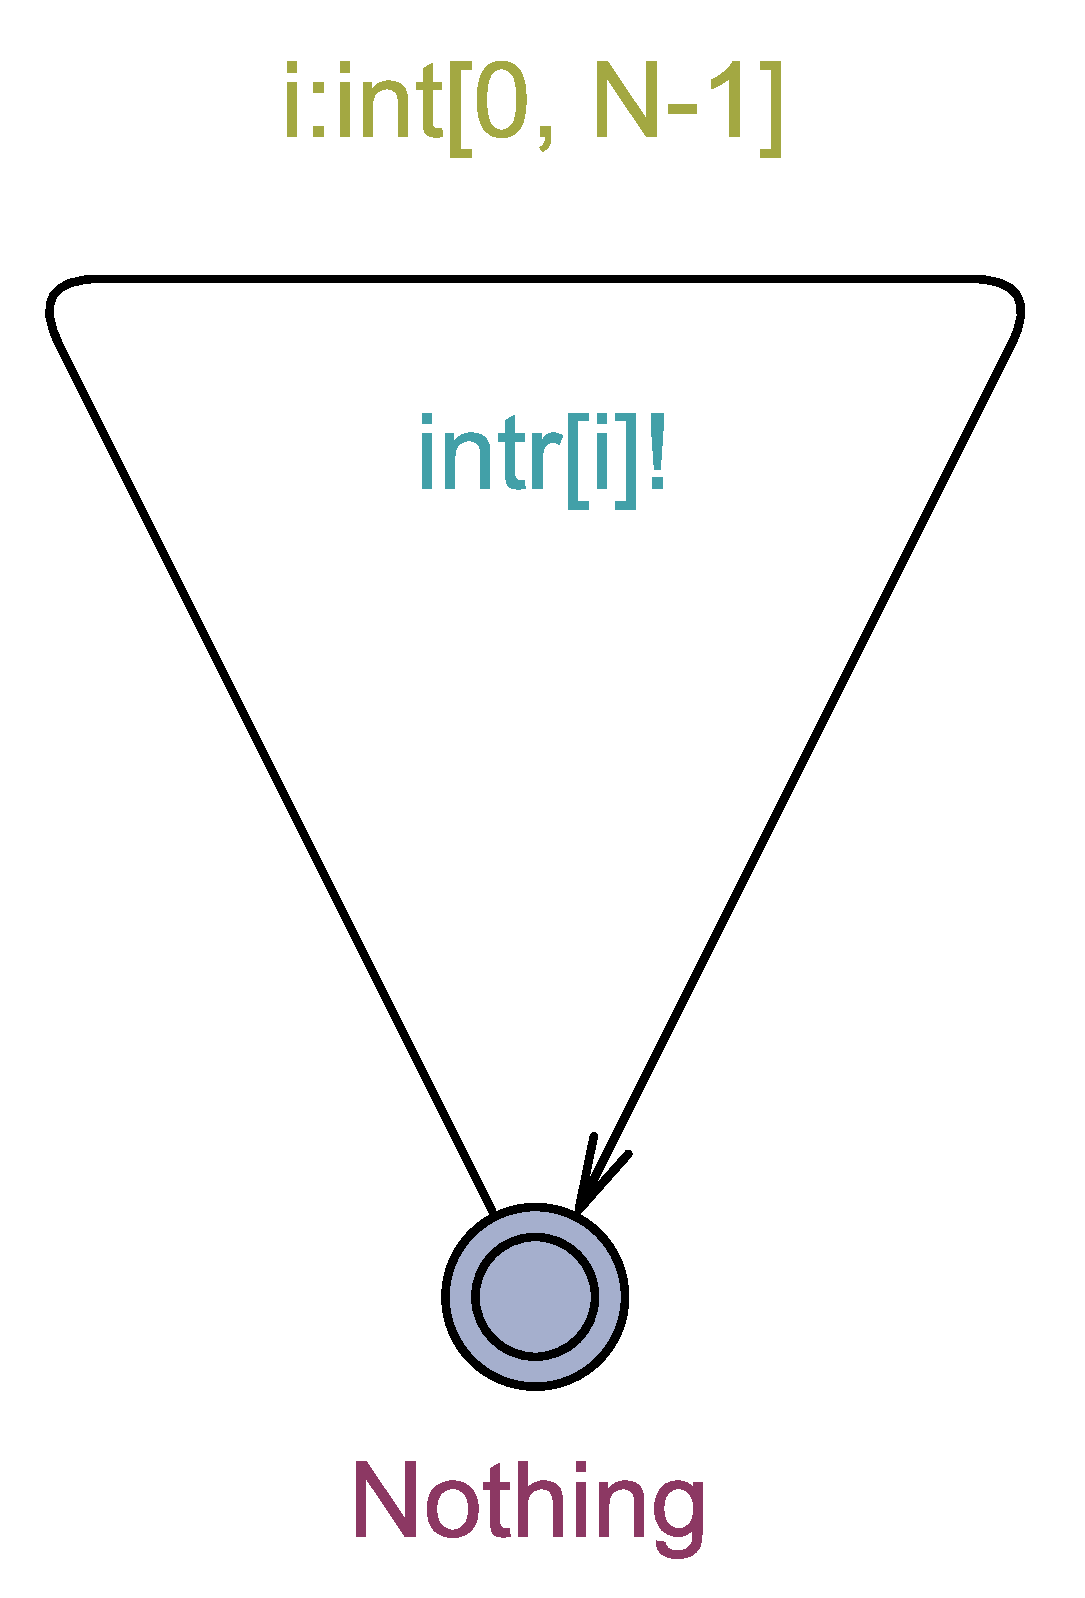
\includegraphics[width=0.2\textwidth]{env_basic}
	\caption{基本中断:环境}
	\label{fig:evn_basic}
\end{figure}

\subsubsection{模型声明}

在模型声明我们将声明所有的实例和模型组成。如图~\ref{fig:basic_model_decl} 所示,
1-7行声明了7个中断实例,注意他们的两个参数,分别对应中断ID和中断处理时间$T$。第9
行生命了中断源。第11行声明了整个模型。至此,我们可以进行仿真模拟,撰写性质交给验
证器去验证。

\begin{figure}[H]
	\centering
	\begin{lstlisting}
	intr0 = Interrupt_basic(0, 1000);
	intr1 = Interrupt_basic(1, 500);
	intr2 = Interrupt_basic(2, 500);
	intr3 = Interrupt_basic(3, 600);
	intr4 = Interrupt_basic(4, 700);
	intr5 = Interrupt_basic(5, 800);
	intr6 = Interrupt_basic(6, 900);
	
	env_basicironment = env_basic();
	
	system intr0, intr1, intr2, intr3, intr4, 
			intr5, intr6, env_basicironment;
	\end{lstlisting}
	\caption{基本中断模型:模型声明}
	\label{fig:basic_model_decl}
\end{figure}

\section{带重入的中断模型}
\label{sec:reentrant}

\subsection{重入的硬件实现}
\label{subsec:reentrant_hardware}

\subsection{Uppaal中的重入中断模型}
\label{subsec:reentrant_uppaal}

\section{分段中断模型}
\label{sec:segment}

\subsection{软件的二次实现}
\label{subsec:segment_software}

\subsection{Uppaal中的分段中断模型}
\label{subsec:segment_uppaal}